% Results, second half: per-update work, capacity, quality, and the predictions that did not hold.
% Every line that carries a number ends in a comment naming the LOG.md entry it comes from.

\subsection{Reducing per-update work}

We measured the five optimizations in the order of Figure~\ref{fig:ladder}, each against an interleaved control that already contains every optimization before it, with 2 repeats per cell. % G11, G12, G13, G14, G16
Each experiment serves $N$ users back to back with a batch size $b$ equal to $N$, at $b=1$ and, for the first four optimizations, at $b=4$. % G11, G12, G13, G14, G16
Table~\ref{tab:ablation} lists the results.

\begin{figure}[t]
\centering
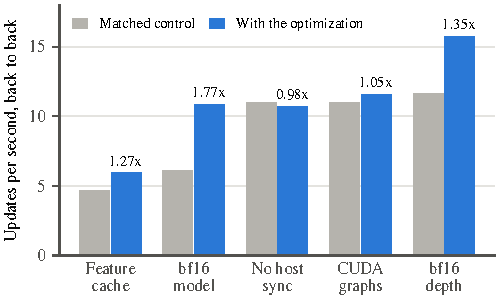
\includegraphics[width=\columnwidth]{figures/ladder}
\caption{Back-to-back throughput at batch size 1 for each optimization (blue) against its matched control (grey), with the ratio above each pair. % G11, G12, G13, G14, G16
Each control contains every optimization to its left.
Each pair comes from its own experiment, so a control need not equal the previous step's result, since runs at different times differ by a few percent. % G12, G14
Bars are means of 2 runs.} % G11, G12, G13, G14, G16
\label{fig:ladder}
\end{figure}

The feature cache, the paper's Algorithm~2~\cite{streamsplat2026}, raises throughput 1.27$\times$ at $b=1$ and 1.21$\times$ at $b=4$. % G11
Running the reconstruction model under bf16 autocast gives the largest single gain, 1.77$\times$ at $b=1$ and 1.95$\times$ at $b=4$, and cuts the model's part of an update from 113 to 46~ms at $b=1$. % G12
The depth model stays outside autocast, and the heads that the authors pin to FP32 stay in FP32. % G12

Dropping the assertions that read values back to the host, and creating tensors directly on the GPU, takes the host waits per cached update from 8 to 0 with bitwise identical output but does not raise throughput. % G13
We kept the change because CUDA graph capture cannot cross a host wait.

CUDA graphs~\cite{nvidia_cuda_guide} record the depth and reconstruction stages once per batch size and replay them.
Capture required turning off block checkpointing, a training-time memory saving that reads the CUDA random-number state even when no gradients are computed.
With checkpointing off in both configurations, the graphs give 1.05$\times$ at $b=1$ and 0.99$\times$ at $b=4$, and their memory pool holds 162--460~MiB more at $b=1$ and 4,152~MiB more at $b=4$, where graphs are recorded for every batch size from 1 to 4. % G14
The effect of turning checkpointing off was not isolated. % G14

After these four steps the depth model, Depth Anything V2 ViT-L~\cite{depthanythingv2}, takes 47~ms of an update, 55--56\% of it, against 37~ms for the rest (Figure~\ref{fig:breakdown}). % G15, G16 (step-0 summary.json: depth 47.1 ms, service 84.2 ms, rest 37.1 ms)
Running it under bf16 autocast, with the interpolation and per-frame normalization of its output kept in FP32, cuts the depth stage from 47.1 to 27.5~ms and raises throughput 1.35$\times$, measured at $b=1$ only. % G16
Measured in the same experiment, \opt{} runs 11.53 updates/s back to back against 4.95 for \serial{}, a factor of 2.33. % G15

\begin{table}[t]
\centering
\footnotesize
\setlength{\tabcolsep}{3pt}
\begin{tabular}{@{}lccccc@{}}
\toprule
 & Updates/s & \multicolumn{2}{c}{Speedup} & Memory & Keyframe \\
\cmidrule(lr){3-4}
Optimization & $b=1$ & $b=1$ & $b=4$ & (MiB) & PSNR (dB) \\ % G11, G12, G13, G14, G16
\midrule
Feature cache & 4.68$\to$5.93 & 1.27 & 1.21 & $+0$ & $0^{a}$ \\ % G11
bf16 model & 6.13$\to$10.83 & 1.77 & 1.95 & $+16$ & $-0.18$ \\ % G12
No host waits & 11.00$\to$10.73 & 0.98 & 1.02 & $+0$ & $0^{b}$ \\ % G13 (memory from outputs/capacity/G13/metrics.json)
CUDA graphs & 10.97$\to$11.54 & 1.05 & 0.99 & $+162$--$460$ & $0^{b}$ \\ % G14
bf16 depth & 11.64$\to$15.71 & 1.35 & -- & $-162$ to $-52$ & $-0.013$ \\ % G16
\bottomrule
\end{tabular}
\caption{Each optimization against its matched control, interleaved in one experiment with 2 repeats per cell. % G11, G12, G13, G14, G16
Updates/s is the mean back-to-back throughput at batch size 1, from control to treatment. % G11, G12, G13, G14, G16
Memory is the change in whole-GPU memory at batch size 1, and for bf16 depth at equal numbers of users in the capacity sweep; the cache's 37~MiB of live tensors per user fit in the allocator's existing reserve. % G11, G12, G13, G14, G16
Keyframe PSNR is the mean change on the DAVIS 2017 validation windows (Table~\ref{tab:quality}). % G12, G16
$^{a}$Not evaluated on DAVIS; the Gaussians match the control's within a mean absolute difference of $4.2\times10^{-8}$ in FP32. % G11
$^{b}$Not evaluated on DAVIS; the outputs are bitwise identical to the control's.} % G13, G14
\label{tab:ablation}
\end{table}

\begin{figure}[t]
\centering
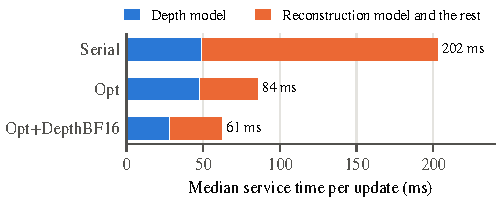
\includegraphics[width=\columnwidth]{figures/breakdown}
\caption{Median service time per update, back to back at batch size 1, split into the depth model and the rest of the update. % G15, G16
\serial{} is one run; \opt{} and \optd{} are each the mean of 2 runs.} % G15, G16
\label{fig:breakdown}
\end{figure}

\subsection{Capacity at one keyframe per second}

We ran the three configurations with every user sending one keyframe per second, under the SLO of Section~\ref{sec:setup} in both repeats.
A first sweep compared \serial{} with \opt{}, and a second compared \opt{} with \optd{} from 10 users upward. % G15, G16
Table~\ref{tab:capacity} gives the result: 4 users for \serial{}, 10 for \opt{} and 14 for \optd{}, each exact on its grid because the next point up was run and failed. % G15, G16
\serial{} reproduces the 4 users that time-slicing and MPS each reached with one container per user (Table~\ref{tab:sharing}). % G6, G15

\begin{table}[t]
\centering
\footnotesize
\setlength{\tabcolsep}{3pt}
\begin{tabular}{@{}lrrrrr@{}}
\toprule
 & Back to back & Capacity & p95 at & \multicolumn{2}{c}{Memory (MiB)} \\
\cmidrule(l){5-6}
Configuration & (updates/s) & (users) & capacity (s) & total & per user \\
\midrule
\serial{} & 4.95 & 4 & 0.205, 0.209 & 3,892 & 973 \\ % G15
\opt{} & 11.53--11.64 & 10 & 0.094--0.100 & 4,928 & 493 \\ % G15, G16
\optd{} & 15.71 & 14 & 0.074, 0.087 & 4,884 & 349 \\ % G16
\bottomrule
\end{tabular}
\caption{Capacity at one keyframe per user per second: the largest number of users for which both repeats meet the SLO.
Back to back is one user at batch size 1 with no pacing, p95 is the worst user's in each repeat at capacity, and memory is the whole GPU's maximum at capacity. % G15, G16
\opt{}'s ranges cover both sweeps.}
\label{tab:capacity}
\end{table}

\begin{figure}[t]
\centering
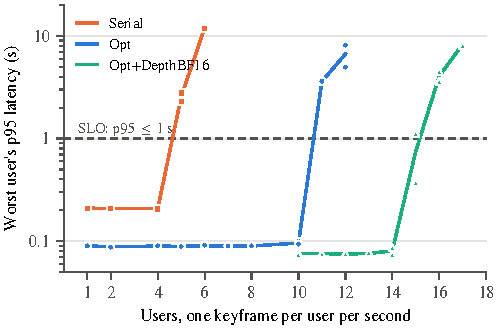
\includegraphics[width=\columnwidth]{figures/latency}
\caption{Worst user's p95 update latency against the number of users, each sending one keyframe per second, on a log scale. % G15, G16
Markers are single repeats and lines join the means.
\serial{} was swept from 1 to 6 users, \opt{} from 1 to 12 and again from 10 to 12, and \optd{} from 10 to 17. % G15, G16
The dashed line is the 1~s SLO.} % G15
\label{fig:latency}
\end{figure}

Below capacity the worst user's p95 stays close to the service time of one update (Figure~\ref{fig:latency}). % G15, G16
At 4 users it is 0.207~s for \serial{} against 0.090~s for \opt{}, and at 10 users 0.097~s for \opt{} against 0.076~s for \optd{}. % G15, G16
Where neither repeat passed, the queue grew for the whole run and the worst user's p95 reached 2.3--12.0~s. % G15, G16
The change is abrupt: at \opt{}'s 11 users the worst user received 57 of 60 updates with a p95 of 3.6~s. % G16

Capacity tracks back-to-back throughput but stops short of it.
\opt{} fails at 11 users, below its 11.64 updates/s, and \optd{} passes 15 users in only one of two repeats, below its 15.71 updates/s. % G16
The SLO held up to about 0.89 of the back-to-back rate (10/11.64 = 0.86 and 14/15.71 = 0.89) and failed from about 0.95 (11/11.64 = 0.945, and 15/15.71 = 0.955 in one repeat of two). % G16
Under overload \opt{}'s median service time also grew, to 96.3--96.7~ms at 11 and 12 users against 84.2~ms back to back, and why the last 5--10\% of the rate cannot be used was not tested. % G16

Memory stayed far from the limit: at capacity the whole card held at most 4,928~MiB, about 10\% of its 49,140~MiB. % G15, G16
All users share one server process and one copy of the weights, so memory per user falls as users are added. % G15, G16
Live tensors grow by 24.6~MiB per user in \opt{}, which we attribute to the cached bf16 features without having measured them separately. % G15
At the largest number of users each configuration ran, nvidia-smi reported a mean GPU utilization of 93\% for \serial{}, 94\% and 84\% for \opt{} in the two sweeps, and 88\% for \optd{}. % G15, G16

\subsection{Quality cost}

Table~\ref{tab:quality} reports quality on the DAVIS 2017 validation set~\cite{davis2017} with the protocol of Section~\ref{sec:setup}. % G8

\begin{table}[t]
\centering
\footnotesize
\setlength{\tabcolsep}{3.5pt}
\begin{tabular}{@{}lrrrr@{}}
\toprule
 & \multicolumn{2}{c}{PSNR (dB)} & \multicolumn{2}{c}{Keyframes vs.\ full} \\
\cmidrule(lr){2-3}\cmidrule(l){4-5}
Precision & keyframes & middle & mean (dB) & $>$0.5~dB loss \\ % G12, G16
\midrule
Paper~\cite{streamsplat2026} & 37.83 & 23.66 & & \\ % G8
Full precision & 37.76 & 23.76 & -- & -- \\ % G8
bf16 model & 37.58 & 23.75 & $-0.18$ & 4.3\% \\ % G12
bf16 model and depth & 37.57 & 23.75 & $-0.19$ & 5.1\% \\ % G16
\bottomrule
\end{tabular}
\caption{Quality on the 1,849 DAVIS 2017 validation windows with the authors' metric. % G8
Full precision is the released code without autocast; the bf16 rows add autocast to the reconstruction model (as in \opt{}) and then to the depth model (as in \optd{}). % G8, G12, G16
The last two columns are paired per window against full precision: the mean change in keyframe PSNR and the share of windows that lose more than 0.5~dB.} % G12, G16
\label{tab:quality}
\end{table}

Running the reconstruction model in bf16 lowers keyframe PSNR by 0.18~dB on average, with per-window changes from $-0.74$ to $+0.20$~dB, while middle-frame PSNR changes by $-0.01$~dB and 0.1\% of windows lose more than 0.5~dB there. % G12
Adding bf16 depth costs a further 0.013~dB of keyframe PSNR, with per-window changes from $-0.26$ to $+0.14$~dB, and 0.0\% of windows lose more than 0.5~dB in that step. % G16
The bf16 DAVIS depth maps differ from the full-precision maps by a mean of 0.36 levels on their 0--255 scale, with a maximum of 36 levels and 67\% of pixels equal. % G16
Against full precision the cumulative loss is 0.19~dB on keyframes, with 5.1\% of windows (94) losing more than 0.5~dB, and 0.01~dB on middle frames. % G16
Rerunning the bf16 evaluation on two sequences reproduced all 64 of their windows bitwise, so the per-window differences carry no run-to-run noise. % G16
The evaluation runs the model's uncached forward pass without CUDA graphs, and its depth inputs differ from the server's in size, 2,442 tokens per DAVIS frame against 1,813 for the test clip, and in precision, FP32 for the full-precision DAVIS maps against TF32 in the server. % G16

\subsection{Hypotheses that did not hold}

Six of the expectations we wrote down before the experiments did not hold.

We expected MPS to serve at least one more user than time-slicing, because a single AnySplat user reconstructing two frames per update showed a mean nvidia-smi utilization of 56\%. % G1
In all four settings both mechanisms served the same number of users (Table~\ref{tab:sharing}), and in the AnySplat settings MPS helped a user measurably only at 5 users, where demand met the throughput ceiling. % G2, G3, G6, G7

We expected batching the updates of 8 StreamSplat users into one call to raise throughput about 2.5$\times$, because nvidia-smi showed the GPU idle 27--36\% of the time at batch size 1. % G5, G9
Batch size 8 gave 0.92$\times$ the throughput of batch size 1. % G9
Under bf16 a batch of 4 cost no more per user than a batch of 1, and we did not test why. % G12

We expected bf16 on the reconstruction model to lower each PSNR metric by at most 0.15~dB. % G12
Keyframe PSNR fell by 0.18~dB, though well inside the 0.5~dB we had set as the largest acceptable loss. % G12
Our untested interpretation is that a small numerical error weighs more against the small remaining error of the keyframes than against the interpolation error of the middle frames.

We expected removing host synchronizations to add 1--5\% throughput, and CUDA graphs to recover about the idle share of the profile, 1.08--1.20$\times$. % G10, G13, G14
They gave 0.98$\times$ and 1.05$\times$ at batch size 1, so neither host waits nor kernel launches account for much of an update, and we did not measure where the GPU's idle time goes. % G13, G14

After the first capacity sweep, in which every tested number of users below the back-to-back rate passed and every one above it failed, we expected the capacity to equal the largest number of users below that rate. % G15
That sweep had not run 11 users, and the second sweep put both optimized configurations one user lower, at 10 and 14. % G15, G16
